\chapter{Evaluation}

In this chapter, we will evaluate the strategies through performance
measurements and discuss advantages, disadvantages and possible use cases.

\section{Performance evaluation}

Performance measurements were taken for each strategy as well as for naive
reference implementations and are presented through latency $lat$ in cycles per
byte (c/B) as well as constant throughput $thr$ in MiB/s of the entire
encryption strategy. Round key derivation is measured separately. Measurements
of all individual components like packing or permuting have to be viewed as
upper bounds due to the aforementioned inlining, instruction reordering and
pipelining (TODO REF HERE) taking place in the actual encryption function.

The AArch64 defines system registers in addition to general-purpose registers
which are used for system configuration and monitoring. One of these registers
is the performance monitor cycle count register \texttt{PMCCNTR} which counts
processor clock cycles. Access from userspace is disabled by default and can be
activated through a custom Linux kernel module by setting \texttt{PMUSERENR.EN}
to 1. To minimize interference and because the cycle count register is
core-local, we isolate and utilize one Cortex-A53 and Cortex-A73 core from the
rest of the system for exclusive benchmarking purposes respectively by use of
the \texttt{isolcpus} kernel command line parameter and \texttt{taskset}
command utility. Results can be found in full in Appendix \ref{app:benchmarks}
and are summarized in Figure \ref{figure:benchmark}.

\begin{figure}[h!]
    \centering
    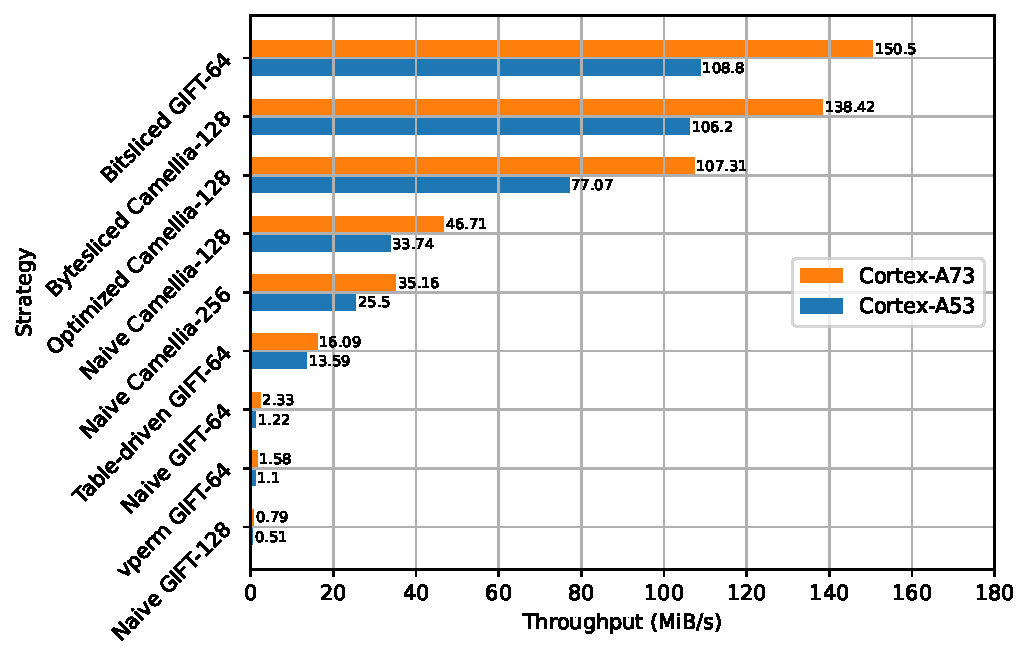
\includegraphics[width=\textwidth]{Figures/benchmark_plot.pdf}
    \caption{Throughput in MiB/s for each strategy and processor type}
    \label{figure:benchmark}
\end{figure}

Bit- and bytesliced implementations leveraging SIMD instructions show the
highest throughput values. Camellia implementations tend to be faster than GIFT
due to the higher number of rounds as well as the bit permutation slowing down
GIFT software implementations, differing from Camellia which is byte-oriented.
Bitsliced GIFT manages to be the fastest due to the bit permutation being
implemented efficiently through bytewise table lookups. Bytesliced Camellia
achieves an only slightly lower performance than bitsliced GIFT in spite of
increased complexity due to the higher number of bytes being encrypted in
parallel.

Table-driven implementations show a $691\%$ and $230\%$ improvement for GIFT
and Camellia respectively compared to their naive implementations. GIFT
especially benefits from this approach due to the elimination of the expensive
bit permutation layer. While S-box lookup is accelerated for \texttt{vperm}
GIFT-64, the whole implementation only achieves a throughput of
$1.58\text{MiB/s}$ due to extremely inefficient packing and unpacking
operations every round.

\section{Conclusion}
